\documentclass[]{article}
\usepackage[utf8]{inputenc}
\usepackage[spanish]{babel}
\usepackage{graphicx}
\usepackage{vmargin}

\setpapersize{A4}
\setmargins{2.5cm}       % margen izquierdo
{1.5cm}                        % margen superior
{16.5cm}                      % anchura del texto
{23.42cm}                    % altura del texto
{10pt}                           % altura de los encabezados
{1cm}                           % espacio entre el texto y los encabezados
{0pt}                             % altura del pie de página
{2cm}                           % espacio entre el texto y el pie de página

%opening
\title{Apuntes para preparar \textsc{Green Belt}}
\author{Nicolás Rodríguez Lucena}

\begin{document}

\maketitle

\part*{Introducción}
\section{Six Sigma y metas organizativas}
Motorola fomenta el Six Sigma a finales de los 80. General Electric de primeras se muestra reticente pero en los 90 le mete mano. 

El fracaso más común es la falta de compromiso por parte de la dirección con la mejora real de los procesos.

\textit{Advanced quality planning (AQP)} para preparar para la implementación de un desarrollo Six Sigma con facilidad, mediante data-driven decisions. 

El especialista en \textit{Quality Control/Quality Assurance (QC/QA)} ha asegurado que los estandares eran establecidos y mantenidos para la satisfacción del cliente. La evolución llevo a apartar al experto QC/QA y darle toda la responsabilidad de la satisfacción de cliente en vez de ser incluida en todos los miembros de la organización. 

\textbf{Shewhart} utilizó gráficos para monitorizar procesos y detectar causas especiales que desviaran los resultados de lo esperado (\textit{quality control charts, process behavior charts}). \newline
Ford en 1988 lanzó el programa \textit{supplier quality improvement (SQI)} para trabajar con proveedores externos en nuevos diseños de vehículos utilizando los \textit{advanced quality planning (AQP)} de la ASQ para mejorar la calidad en el ensamblaje, todo esto dio lugar al \textit{advanced product quality planning (APQP)} que se utiliza en la industria automotriz. 

Motorola le presentó el Six Sigma a Ford y lo evaluó contra Ford Q1 y Q-101 (precursor de ISO/TS 16949). Solo un punto que no le gustó, estaba establecido el $C_p$ en 1.0. Ford quería $C_{pk} >$ 1.33 para procesos conocidos y $C_{pk} >$ 1.67 para los nuevos.

Six Sigma: reducir la variación y mejorar el control del proceso. Lean: expulsa residuos y promueve el estandarizar trabajos. 

\textbf{Subir Chowdhury}: los problemas pueden ser evitados a través de la mejora continua, la calidad es responsabilidad de todos los individuos, la calidad empieza arriba, todos tienen un papel en la calidad, la calidad es el balance entre el poder de la gente y del proceso. Poder de la gente necesita compromiso, honestidad y empatía. Process power es solucionar problemas, desarrollar ideas y soluciones. Toda organización es única, cada individuo trae diferente conocimiento y habilidades. Métodos y procesos deben ser desarrollados para cada específica situación.

\textbf{Philip Crosby}: Sus 14 pasos. 1) Gerencia comprometida con la calidad 2) Equipos de mejora continua con miembros de todos los departamentos 3) Determinar como medir donde están los problemas 4) Evaluar el coste de calidad 5) Incrementar la conciencia de calidad en la organización 6) Tomar acciones formales para corregir problemas identificados en pasos anteriores 7) Poner un comité de 0-defectos 8) Formación para todos 9) Establecer el día "cero defectos" 10) alentar a que la gente establezca metas de mejora para ellos y para sus grupos 11) alentar a la gente a que comente los problemas de gestión 12) reconocer y apreciar la participación de la gente 13) establecer "Consejos de Calidad" para comunicarse de manera regular. 14) Re-run el programa desde 0, para que la gente vea que esto nunca se acaba. 

\textbf{W. Edwards Deming}: Otros 14 puntos. 1) constancia en la mejora 2) nueva filosofia 3) no todo es inspección 4) no todo es precio 5) mejora constante para planificación, producción y servicio 6) formacion 7) liderazgo 8) evitar miedos 9) quitar barreras entre el staff 10) fuera el trabajo duro 11) quitar ránkins y mierdas para cuantificar trabajo duro y metas de gestión 12) quitar barreras que roben a la gente el orgullo del trabajo. Sistemas de méritos etc.. 13) Plan de Formación y mejora personal 14) Todos para realizar el cambio. Y sus 7 enfermedades mortales: 1) falta de constancia 2) el cortoplacismo 3) evaluacion por meritos y mierdas 4) Movilidad de la direccion 5) el funcionamiento basado solo en 'figuras visibles' 6) costes medicos excesivos 7) jugar en el borde de la ley. 

También preparó el \textit{Sistema del conocimiento profundo}: 1) Apreciación de un sistema (process aproach) 2) Conocimiento de la variación (existe, como reconocerla). 3) Teoría del conocimiento (how to learn) 4) Conocimiento de la psicología (Maslow, Regla de Platino...) 

\textbf{Armand Feigenbaum}: Planifica y transmite el plan. Planificar es bien ya que el propósito de la planificación es 'hacerlo bien'. En tres pasos: Liderazgo de la calidad, tecnología moderna de la calidad y comité de organización. Los planes AQP son suyos. 

\textbf{Kaoru Ishikawa}: Diagrama causa-efecto. Trabajó con Deming a tope. Sus puntos: Calidad primero, por delante de rentabilidad corto placista. Orientar hacia cliente (pensar desde su POV). El siguiente proceso es el cliente (que haya feedback). Hechos y datos, estadística. Humanidad como filosofía de gestión. Gestion interfuncional. 

\textbf{Joseph M Juran}: quality planning, quality control y quality improvement. Sus puntos: crear conciencia, la calidad es de todos, haz una infraestructura de calidad (council, appoint teams, ...), formación sobre Calidad, revisiones periodicas, reconocimiento a los equipos ganadores, revisar el sistema de recompensas para hacer cumplir el ratio de mejoras, mantener un plan de negocio basado en la mejora de la calidad. Pareto es suyo. 

\textbf{Dorian Shainin}: ing. aeronautico que desarrolla soluciones para los problemas mas dificiles. Habla con las \textit{parts}, son mas listas que los ingenieros. Invento la Red X.

\textbf{Walter Shewhart} trabajador de Western Electric inventó el PDCA y es el padre del control estadístico de proceso. 

\textbf{D. H. Stamatis}: 45 libracos sobre Six Sigma, calidad y demás. El Manual del FMEA es suyo y la documentación del Six Sigma.

\textbf{Genichi Taguchi}: Inventó la Loss Function, usada para medir el coste financiero por empeorar la calidad y desarrolló la filosofía de \textit{off-line quality control}. 

\textbf{Proceso}: serie de pasos diseñada para producir productos o servicios. A menudo representado como un diagrama de flujo con inputs (materiales, recursos, info), steps, y hay un output. Para aplicar Six Sigma, se meten los pasos del DMAIC (\textit{define, measure, analyze, improve y control}). 

\textbf{Business Systems}: diseñados para implementar un conjunto de procesos. Se asegura de que todo esté en el lugar adecuado en el momento adecuado. Tiene como meta la mejora continua de proesos, productos y servicios. Se encarga de recoger y analizar la información de los procesos y de otras fuentes para la mejora continua.  

Hay dos maneras de ver el método utilizando inputs / recursos para producir resultados de calidad: la gestión de procesos es recoger datos y analizarlo, aplicando el feedback al proceso. Por otro lado se piensa que el proceso debe ser diseñado orientado hacia la colección de datos, análisis y el feedback que se va a producir.

Man, Machine, Methods, Mother Nature, Management, Materials, Measurement System para Productos y/o Servicios.

Métodos alternativos al Six Sigma: Quality Operating System (QoS), mejora contiuna (CI), total quality management (TQM), mejora de procesos (PI), Reto: revisar procesos para mejoras: mantenimientos preventivos, limpieza, desgaste...

La línea general es: qué medir, cómo medirlo, es fundamental el proceso?, consenso sobre defectos, exponer defectos latentes, observar la calidad estadística (cartas de comportamiento de proceso), distinguir entre Calidad de Diseño y Calidad de Conformidad. 

\subsection{Modelo DMAIC}
Define: PDCA, SIPOC, 5W, Systems thinking, Process Identification, Flowchart, Project Management. \newline
Measure: PDCA, Data collection plan, Measurement systems analysis (MSA), Collect Data (check sheets, histograms, pareto charts, scatter diagrams), identificar variabilidad-instabilidad, benchmark, start cost of quality. \newline
Analyze: PD\textbf{S}A, mejora continua, mantenimiento preventivo, limpieza, benchmark, teorema del limite central, GD\&T, shop audit, experimentos. \newline
Improve: PD\textbf{S}A, mejora procesos, desarrollo organizacional, reducción de la variación, solución de problemas, brainstorming, flowchars 'should be', FMEA, coste de calidad, diseño de experimentos. \newline
Control: SDCA, plan de control, dynamic control plan (DCP), MSA largo plazo, mistake-proofing, process behavior charts.

\subsection{Six Sigma Road Map}

\begin{enumerate}
	\item Existe la variacion en todo. Hay que estandarizar el trabajo.
	\item Identifica lo que el cliente quiere y necesita. Reduce variación.
	\item Metodo problem-solving para mejorar los planes.
	\item Seguir el DMAIC para desarrollar la mejora.
	\item Monitorizar el proceso con Process Behavior Charts.
	\item Subir de nivel el estandar de los procedimientos y lecciones aprendidas.
	\item Celebrar el exito
	\item Empezar de nuevo con la mejora continua PDSA/SDCA.
\end{enumerate}

\subsection{Cost-Benefit Analysis}

Muchas cosas que funcionan en una tienda se pueden clasificar en: \textit{prevention cost}, appraisal costs (evaluacion), costes de fallos internos y costes de fallos externos. 
Cuando se calculan los costes de calidad en un negocio se plotea una curva tal como Fig \ref{fig:CurvaCostesdeCalidadInicio}.
\begin{figure}[ht!]
\centering
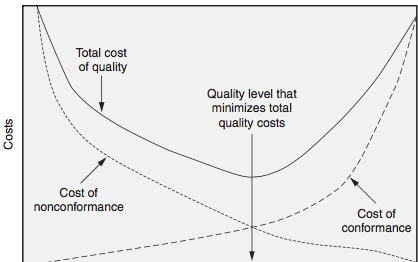
\includegraphics[width=90mm]{imagenes/CurvaCostesCalidadInicio.png}
\caption{Curva de Costes de Calidad antes de iniciar el desarrollo}
\label{fig:CurvaCostesdeCalidadInicio}
\end{figure}

En la primera ronda de medidas de costes nadie debe ser increpado, debe servir a modo comparativo y para sacar el qué hacer y el cómo hacerlo. La meta es intentar llegar a la Fig \ref{fig:CurvaCostesdeCalidadFin}.

\begin{figure}[ht!]
	\centering
	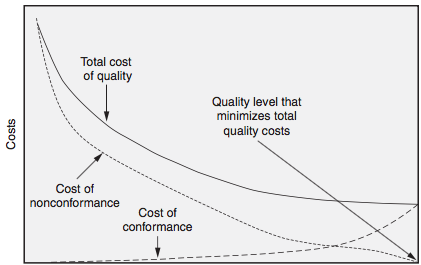
\includegraphics[width=90mm]{imagenes/CurvaCostesCalidadFin.png}
	\caption{Curva de Costes de Calidad al final del desarrollo}
	\label{fig:CurvaCostesdeCalidadFin}
\end{figure}

Una técnica para desarrollar estrategias es la planificación \textit{hoshin}. Desarrollar 4 visiones de lo que debería ser la compañía en 5 años.

Expected Profit = $\sum$ Profit x Probability

Cuando un sistema trabaja por debajo de su nivel óptimo es \textit{suboptimization}.

\subsection{Conductores de la organización y métrica}
Factores clave: hay que sacar datos e información de clientes, productos, servicios, operaciones, mercado, competitividad, proveedores, sindicatos, costes, gobiernos y cumplimiento del rendimiento. Indicadores.

\textbf{Voice of the Customer (VoC)}: factor clave el cliente y el conocimiento del mercado. Las relaciones con clientes y la habilidad de determinar cómo adquirir un nuevo cliente, satisfascerlo, conseguir su lealtad para retenerlo y expandir el mercado. VoC es el proceso para capturar información relacionada con los clientes. La intención es anticiparse a los requerimientos de cliente, necesidades y deseos. La meta es conseguir la lealtad para construir relaciones entre-con clientes. VoC puede incluir reunir e integrar datos de encuestas, datos de la web, datos de garantías, registros de quejas y toda aquella información que afecta a la compra y a las decisiones que toma un cliente.

\textbf{Balanced Scorecard (BS)} (tarjetas de puntuación): miden desde rezagadas hasta líderes las areas: financieras, cliente, procesos internos, y carrera del empleado. Las medidas rezagadas son aquellas al final del evento y las lideres son las que ayudan a conseguir objetivos y se miden antes del evento. 

Este método sirve para saber que es lo que tienen que medir las compañías en orden de equilibrar los resultados financieros. 
BS no es solo un sistema de medida, también es un sistema de gestión que permite a las organizaciones focusear su visión y estrategia convirtiéndolas en actos. Provee feedback en procesos internos y externos. Una vez completamente integrado, el BS convierte el plan estratégico en el centro nervioso de la empresa.

\textbf{Scoreboard/Dashboard}: representación visual que da una visión rápida de la compañía a tiempo real. Es crítico para ayudar al empleado a predecir ventas, cash flow, beneficio y da claridad a la actuación y dirección de la compañía. Debe ser una herramienta crítica de toma de decisiones usada en las operaciones del día a día. Tres pasos para construir un efectivo \textit{Dashboard}: 1) conocer los promedios y el benchmark de la industria. 2) conocer nuestra posición y trayectoria sobre estos promedios y el benchmarking 3) desarrollar cada llamada al BS en un conjunto comprensivo de la compañía, no solo las partes implicadas.

\textbf{Key Performance/Process Indicator (KPI)} (indicador clave de rendimiento): Medida cuantificable que acordada de ante mano, refleja el éxito de los factores críticos. Hay que saber elegir que medidas necesitas trackear/perseguir en tus proyectos. 

\section{Principios Lean en la organización}

Lean: valor, waste y el proceso de crear valor sin waste. Añadir valor sin reducir nada mas es la idea. Toyota Production System es el origen y la clave del Lean. La casa del TPS es lo suyo. Supongo que mas adelante se verá más claro.

\begin{figure}[ht!]
	\centering
	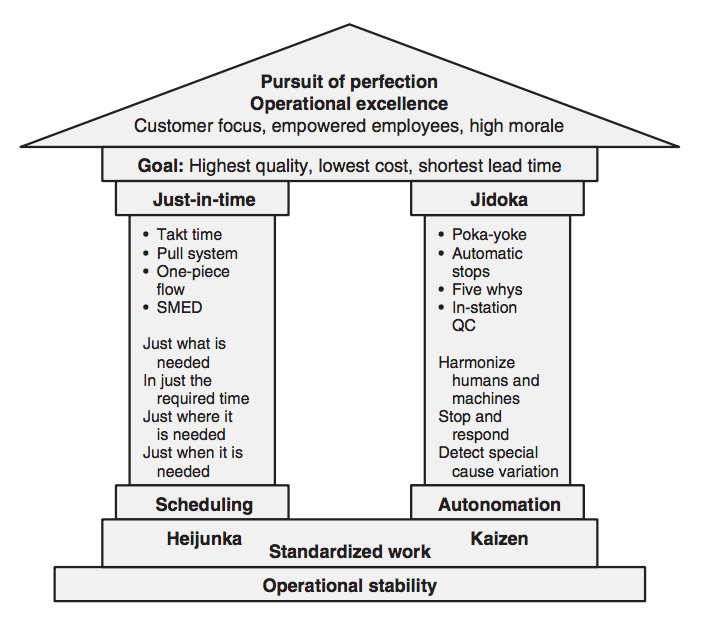
\includegraphics[width=120mm]{imagenes/TPSHouse.png}
	\caption{TPS House}
	\label{fig:TPS House}
\end{figure}

\subsection{Value}

El concepto que mas preocupa a los negocios en los años recientes es \textit{valor}. La percepción de la utilidad y necesidad de un producto o servicio. 

La gente coge coches japoneses por calidad, confianza y eficiencia. La gente coge coches alemanes por otros valores, el orgullo de marca por ejemplo. Los coches americanos son comparables con ambos, pero ellos creen en la lealtad del cliente. 

Un paso tiene valor añadido dentro de un proceso si: el cliente reconoce el valor del producto/servicio, si esto transforma el producto, si está bien hecho a la primera.

Non-value-added, rework, son actividades por las que el cliente no está dispuesto a pagar. El cliente está dispuesto a pagar por la impresión de un documento pero no por las correcciones del proveedor. "question everything" para buscar actividades non-value-added. Siempre hay zonas grises entre valor añadido y no valor añadido. Esto ocurre con inspección y testeo. El cliente no quiere problemas, por lo que inspección es valor añadido, pero la solución es mejorar el proceso hasta el punto de que no tenga que ser inspeccionado. Por otro lado, el sello de la IFS da categoría, así que hacer lo que el sello pida es lo suyo, ya que tenerlo da un valor añadido.

Los 14 principios del Camino Toyota: 1) decisiones de gestión en una filosofía de largo plazo. 2) proceso continuo que lleve los problemas a la superficie. 3) pull system para evitar overproduction 4) nivel de carga de trabajo 5) construir cultura de parar a arreglar problemas para tener calidad desde el primer momento 6) estandarizar tareas y procesos 7) controles visuales 8) tecnología fiable y probada 9) crecer lideres que entienden el trabajo a fondo, viven la filosofia y enseñan a otros 10) desarrolla gente y equipos que sigan la filosofia de la compañia 11) respeta la red de compañeros y proveedores retandolos y ayudandolos a mejorar 12) ve y mira por ti mismo para entender la situacion 13) toma decisiones en concenso y teniendo en cuenta todas las opiniones 14) empieza una organización que aprenda la mejora continua.

\subsection{Herramientas Top Lean}

\textbf{5S (o 6S, o 7S)}. Método de organización del lugar de trabajo para mejorar la eficiencia. El orden: \textit{Sort}: Lo que no hace falta o rara vez hace falta, fuera. Muchas cosas da lugar a desorden y desorden da lugar a pérdida de tiempo. \textit{Set in order}: Colocación de las cosas necesarias en el sitio necesario: instrucciones, herramientas, gafas de seguridad. \textit{Shine}: la limpieza es importante. Una vez resuelto (si es un ejercicio intelectual) hay que dejarlo bien organizado y limpio para que se entienda, esa es la filosofía de la limpieza. \textit{Standarize}: desarrollar checklist, starndarts e instrucciones de trabajo para tener un orden. \textit{Sustain}: mantener las otras 4 S. Las 5S mejoran la productividad y la eficiencia, reduce los accidentes. La gestión debe dar poder a los empleados para que ellos puedan propiedad de sus areas de trabajo. Las otras dos \textit{Safey}-seguridad y \textit{Oversight}-asegurar a la primera.

\begin{figure}[ht!]
	\centering
	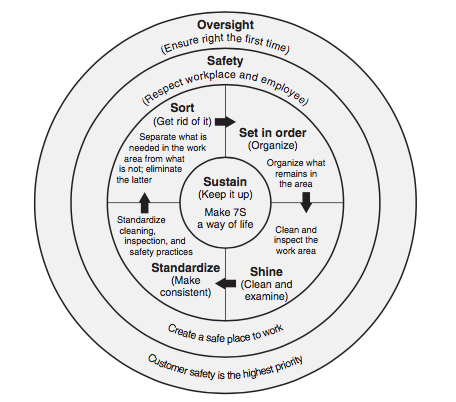
\includegraphics[width=90mm]{imagenes/7S.png}
	\caption{7S adaptation}
	\label{fig:Las7S}
\end{figure}


\textbf{Andon}. Sistema de feedback visual (semáforo) para advertir del nivel de calidad de producto.

\textbf{A3}. Un formato a 3 que contenga: Antecedentes, Situación Actual, Análisis de Causas, Objetivos de Mejora, Acciones de mejora, Plan de acción, Seguimiento de los resultados. No todos los problemas necesitan un A3, solo los complejos y no-evidentes.

\textbf{Gemba}. Ir a planta, allí es donde ocurren las cosas!. Gestión mientras caminas.

\textbf{Heijunka}. Calendario productivo orientado en hacerlo en pequeños bloques de secuencias, en el mismo proceso. Para reducir tiempos muertos y tener bajos niveles de inventario.

\textbf{Hoshin Kanri}. Quality Function Deployment. Consiste en alinear las metas de la compañía (strategy) con los planes a medio plazo (tactics) y las operaciones de trabajo (actions). 

\textbf{Jidoka (Autonomation)}. Por qué hacerlo a mano si una máquina lo puede hacer mejor. Sobre todo si son cosas tediosas. 

\textbf{Kaizen Continuous Improvement vs Kaizen Events}. Mejora continua. \textit{Kaikaku} es un evento Kaizen. Resultados rápidos. Apoyo de la gestión para cada iniciativa. Si los empleados no pueden mejorar el proceso entre 3 - 5 días, la organización necesita reajustar la cultura.

\textbf{Kanban (Pull System)}. El sistema es mejor controlado cuando material e información fluye hacia dentro y fuera de los procesos de manera suave y racional. Ocurre que muchas veces llega antes de tiempo, informacion confusa... Un sistema Kanban da la información necesaria en el momento oportuno. Funciona usando unas visual cards.

\textbf{Overall Equipment Effectiveness (OEE)}. El concepto de medir la efectividad de una operación: \textit{availability, performance and quality}. A * P * Q. 

\textbf{Single Minute Exchange of Die (SMED)}. Rápido y efectivo camino para convertir un proceso operativo en un producto hacia el siguiente. Los grandes cambios son la clave para reducir lotes de producción. \textit{Pensar en esto para Lean Office}.

\textbf{Standar Work}: 9001 es la ley para esto. Poco que decir, crear mapa de procesos, y esas cosas.

\textbf{Takt Time} del aleman \textit{taktzeit}. La batuta de una orquesta. Goles, velocidad, tiempos. Ajustar producción con demanda.

\textbf{Theory of Constraints}. Metodología de problema-solución que busca el enlace más debil de la cadena. Normalmente es el mas lento. Identificar, Explotar (mejorar), Subordinar (el resto a este), Elevar (revisiones, inversiones, mejora del weak) y Repetir.

\subsection{Muda}

El waste (muda) viene de varias fuentes. Cuales?

\textbf{Overproduction}. Hacer mas de lo que necesita el siguiente proceso. Principal síntoma \textit{Work In Process WIP}.

\textbf{Excess motion}. Workplace layout. Ergonomic problems, tiempo gastado buscando o moviendo provisiones o equipo.

\textbf{Waiting}. Esperas, setups largos, gente que no aparece, la gente se demora. 

\textbf{Inventory}. Tienes inventario? el control sobre él es un gasto. Equilibrio control de stock vs ciclo económico, retorno de la inversión.

\textbf{Excess Movement of Material/Transportation}. Los movimientos de handling y storing matan. Un plant layout bien puesto para evitar esto. Function-oriented departments necesita muchos movimientos.

\textbf{Defect Correction}. Corregir defectos. Actividad non-value added. Tipicas causas: mal equipo de mantenimiento, mal sistema de calidad, malas instrucciones de trabajo y mal diseño. 

\textbf{Excess Processing/Overprocessing}. Dificiles de reconoces. Demasiados procesos. 

\subsubsection{Otros}

\textbf{Falta de creatividad}. Empleados tienen que tener ideas para mejorar los procesos.

\textbf{Perfeccion}. Evitar la perfección exacta. 

\subsection{Value Stream Mapping} 

\textit{Value Stream} es una serie de actividades que hace una empresa: pedir, diseñar, producir, entregar productos/servicios. Un value stream empieza por los proveedores de los proveedores y acaba con los clientes de los clientes. Componentes: 1. Flow materials desde proveedor hasta entrega a cliente (los pedidos entran semanalmente en camion, los materiales se mueven hasta la zona de produccion y al almacen de producto terminado, producto terminado se entrega a cliente), 2. Transformation of raw materials (pasos de produccion rollo cortar, moldear, forjar...), 3. El flujo de información requerido para ayudar al flujo de material y a la transformación (ordenes de compra a provedores, ordenes internas de trabajo, shipping notice...).

Value Stream Map usa gráficos con iconos simples para ilustrar el movimiento del material, inventario, work-in-progress, operadores... Un Value Stream Analysis es el que descubre \textit{wastes} ocultos en la organización. Aplicar Lean Thinking para dividir un \textit{path} en diferentes pasos: 1. Producir un \textit{value stream map (value chain diagram)}. 2. Analizar las notas de inventario pensando en reducirlo o eliminarlo (inventario = coste del espacio, perdida de calidad, V2 v3 v4..., el dinero se puede invertir en otras cosas), 3. Analizar los non-value steps para eliminarlos, 4. Determinar como es conducido el flujo (p.e.: en funcion de pedidos del cliente), 5. Extender el value stream map hasta los proveedores (compatibilidad entre sistemas-codigos de barras).

\begin{figure}[ht!]
	\centering
	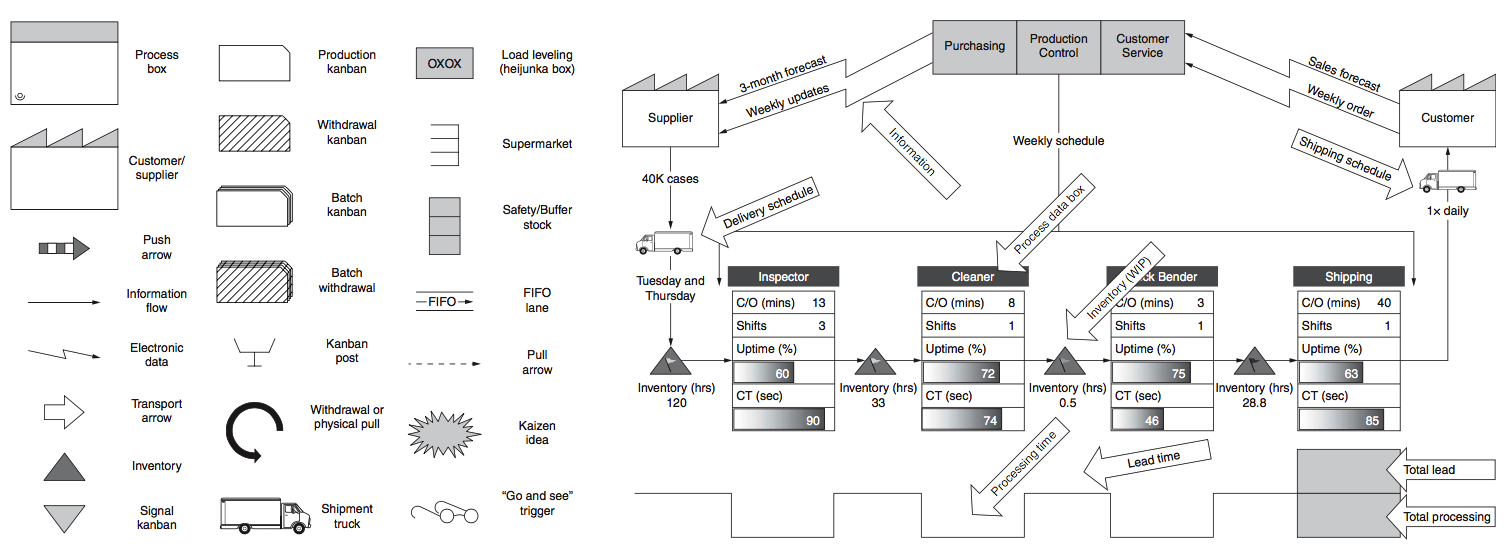
\includegraphics[width=170mm]{imagenes/ValueStreamMapping.png}
	\caption{Value Stream Mapping}
	\label{fig:ValueStreamMapping}
\end{figure}

\section{Diseño para metodologías Six Sigma (DFSS)}

DFSS se apoya proceso estratégico de negocio/ingenieria y en procesos capaces de reducir y gestionar variaciones: con DMADV (define, measure, analyze, design, verify) y con IDOV (identify, design, optimice, verify). Hay batiburrillo de sigmas DFSS, DCOV, ICOV, DMEDI, IDDOV, GD. Se use el que se use, pero hay que recordar: robustez del sistema usado, no abrir mil proyectos, uno para cada síntoma, evitar perder el tiempo alimentando el sistema de datos y ratings, alcance vago o pequeño. Lo que no puedes controlar se llama \textit{noise}. \textit{noise strategy} para mejorar el proceso.

Usamos DFSS para aumentar la satisfacción de cliente, reducir variaciones, tener un diseño robusto, bajar costes de garantía, mejorar durabilidad, incrementar facturación-ganancias y producción (ésta última a través de bajar downtimes por defectos).

\subsection{IDOV} \textit{Identify} \textit{Design} \textit{Optimize} \textit{Verify} similar al MAIC del Six Sigma (\textit{measure, analyze, improve, control}).

\textit{Identify Phase}: identificar requisitos de producto y cliente, establecer caso de negocio, identificar aspectos técnicos, critical to quality (CTQ) variables, y limites de especificaciones, roles y responsabilidades, hitos.

\textit{Design Phase}: Formular el concepto, identificar posibles riesgos usando FMEA (failure mode and effects analysis), para cada detalle técnico, identificar parámetros diseño, usar DOE (design of experiments) y otras herramientas de analisis para determinar CTQs y su influencia en los requisitos técnicos.

\textit{Optimize Phase}: Evaluar las posibilidades del proceso y llegar a conocer bien los limites CTQ. Optimizar el diseño minimizando los CTQs, prueba-error, estadisticas y tolernancias.

\textit{Validate Phase}: Prototipado, evaluar actuacion, fallos, confianza y riesgo, design iteration y revisión final de producto.

\subsection{DMADV} Para cuando el producto no existe y ha de ser desarrollado. O ya existe pero no se conocen las necesidades del negocio o del cliente. 

\textit{Define}: Targeting prioridades.

\textit{Measure}: combinación de análisis técnico y competitivo del producto. 

\textit{Analyze}: Aproximaciones de estadística e investigación, para establecer prioridades y confianza.

\textit{Design}: Design for/to Cost: busqueda de alternativas en procesos, materiales, métodos... Design for Manofacturing/productibility/assembly: pequeños cambios que hacen que sea mucho mas barato fabricarlo. Design for test: donde testing es critico, lo mejor es hacer test tempranos en el ciclo de producción. Design for maintability:si necesitas muchos downtimes y reparaciones. Design for Robustness: test en todos los ciclos de vida, y partes, ensamblajes y sub. Design for usability: VALIDATION!  puede ser medido y mejorado. Extended for functionality: otras features desde el pto de vista del diseño. Design for efficiency: consumo minimo de recursos. Design for Performance: la mejora de los microchips es un ejemplo. Design for security: preserva la integridad del producto. Design for scalability: 

\textit{Verify}: Es necesario asegurar los resultados del diseño de los objetivos. 

\subsection{FMEA} Usa FMEA para evaluar el proceso o el producto y determinar que causa el fallo y los efectos que pueden tener. 
Identifica y usa escala, calcula el Risk Priority Number (RPN) y analiza los resultados.

La esencia del \textit{failure mode and effects analysis} es el estudio del riesgo. Riesgo es lo incierto de un evento. Riesgo es la posible influencia buena o mala de un producto en un entorno. El riesgo se puede definir como impact (severity)  probability (ocurrence) y event (detection). Segun Risk Road Map ISO 31000:2009: gestión del Plan risk / herramientas del risk identification / analizar y evaluar riesgos / plan risk response / monitor y control del risk.

\begin{figure}[ht!]
	\centering
	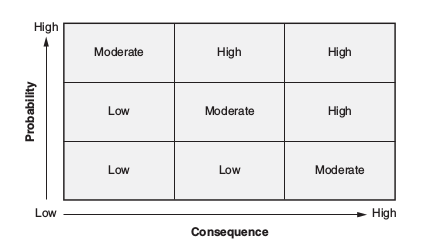
\includegraphics[width=90mm]{imagenes/RiskMatrix.png}
	\caption{Risk Matrix}
	\label{fig:RiskMatrix}
\end{figure}

FMEA es una herramienta front-end. Un producto/proceso de éxito requiere anticiparse a los problemas y para ello hace falta tener jerarquizados cuales atacar antes, y/ como atacarlos. \textbf{Mirar Effective FMEAS}. El documento de gestión FMEA se tiene que ir controlando por versiones, incluyendo y quitando cosas, ya que es un documento vivo. Beneficios del FMEA: evaluación a todos los clientes (internos y externos), ayuda en la evaluación de requerimientos y alternativas, ayuda a centrarse en donde pueden aparecer los problemas criticos y como paliarlos/evitarlos/controlarlos, desarrollo de una lista de actuaciones priorizada, ayuda para evaluar el propósito del proceso.

\begin{figure}[ht!]
	\centering
	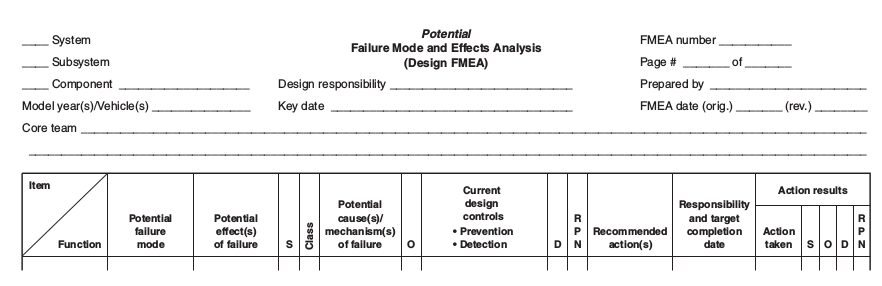
\includegraphics[width=170mm]{imagenes/PlantillaFMEA.png}
	\caption{Cabecera de una plantilla FMEA}
	\label{fig:PlantillaFMEA}
\end{figure}

\begin{figure}[ht!]
	\centering
	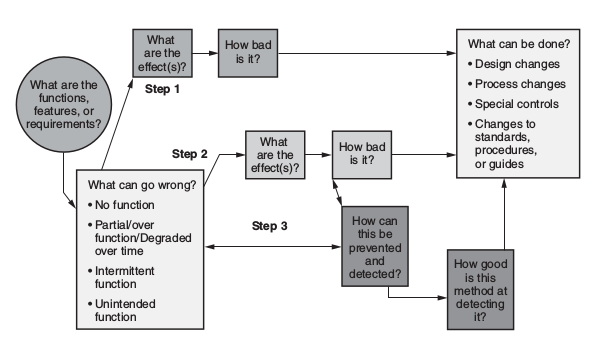
\includegraphics[width=90mm]{imagenes/FMEAFlowchart.png}
	\caption{Diagrama de flujo de FMEA}
	\label{fig:FMAFlowchart}
\end{figure}

Pasos del FMEA: 1. Lista los pasos claves de un proceso 2. brainstorm de porque puede fallar cada paso 3. lista de efectos de los fallos 4. ranking de severidad para los efectos 5. causa y frecuencia de los fallos 6. controles para la detección 7. calcular RPN 8. Ordenar por críticos los RPN. 9. Desarrollar plan de accion, asignando persona-responsabilidad 10. Re-Calcular el RPN una vez implantado.

\subsection{Do's} 1. Da formacion de FMEA antes de asignar equipos 2. Enfoque de equipo 3. Pregunta a expertos si es necesario 4. Habla con el cliente de como va a utilizar el producto 5. brainstorm de los posibles fallos. 6. Si dos riesgos tienen la misma RPN, se queda encima el que tenga mas severidad. 7. completa la accion y reasigna la severidad. 8.Actualiza el FMEA con los nuevos riesgos aprendidos.

\subsection{Don'ts} 1. No copies el S-O-D de una industria a otra. 2. Intenta no usar una escala de 1-10, de 1-5 mejor. 3. No hagas escalas especializadas sino es completamente necesario. 4.	No manipules los datos.

\begin{figure}[ht!]
	\centering
	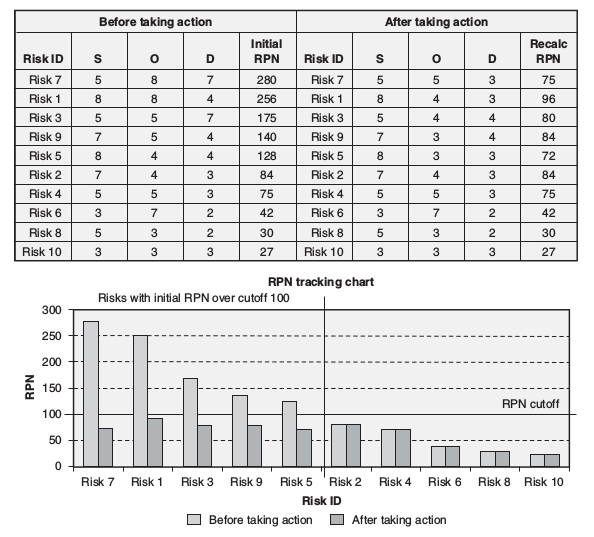
\includegraphics[width=140mm]{imagenes/FMEAPrePos.png}
	\caption{Report final de un FMEA}
	\label{fig:FMEAPrePos}
\end{figure}

\part*{Definicion}

Preguntas críticas de la fase de definición: donde estamos? cual es el problema? donde queremos estar? como vamos a llegar allí? como sabremos que hemos llegado a ese punto?

Antes de empezar, comprobar que la gestión y la economía del proyecto están alineadas. Mas tiempo frente a una buena planificación, mayor será el éxito. 

\section{Identificación del proyecto}
\subsection{Project Selection}

Describir el proceso de seleccion de proyecto y que factores deben ser incluidos para considurar si usar DMAIC u otro tipo de problem-solving process. Lo suyo es que haya un departamento o comité para decidir qué proyectos se pueden llevar a cabo y cuales no, ya que todas las ideas a la vez son imposibles. Cada propuesta debe tener medidas sobre el problema que plantean resolver y el impacto de éstas sobre la organización. Managers suelen coger la que ahorre más dinero a la compañía.
Proyectos que tengan que ver con el análisis de datos, para el equipo de Six Sigma. Los que tengan que ver con mejora de procesos, con el equipo de Lean Manufacturing.

\subsection{Process Elements}

Definir y describir los componentes del proceso	y límites (boundaries). Reconocer como los procesos cruzan varias areas funcionales y los retos que resultan de los esfuerzos de mejora de procesos. Los procesos se pueden subdividir en subprocesos.
Por ejemplo, el proceso de payroll tiene subprocesos: reunir la información del reloj de fichar, hacer deducciones, ...

Para definir bien un proceso hay que marcar donde empieza y donde acaba. Los límites (boundaries). Los procesos transversales pueden tener subprocesos límite, definidos por la estructura del negocio, geografía...

\subsection{Benchmarking}

Entender que hay varios tipos de benchmarking, incluyendo la competitividad, la colaboración y las buenas prácticas.
Pueden ser internas, contra otros procesos internos o externas. Las fuentes de información del Benchmarking vienen de publicaciones, reuniones profesionales, investigaciones universitarias, feedback de clientes, visitas, análisis de productos de competidores...

Operaciones de Benchmarking: analizar la operativa, conocer los líderes del mercado, incorporar lo mejor de lo mejor, ganar superioridad. 

Internal benchmarking: facil acceso a otros dptos. sin embargo, el límite de mejora está reducido al estilo de la compañía.

Competitive benchmarking: fuerza a la compañía a tener una perspectiva externa. Sin embargo, fijarse en las prácticas de las industrias puede limitar el alcance de altos niveles de actuación.

Funcional benchmarking: comparas funciones similares, normalmente se busca fuera de la empresa y permite conseguir más partners de benchmarking.

Collaborative benchmarking: cooperación entre varias organizaciones para lograr resultados de benchmarking. Esta práctica permite el acceso a benchmarking partners  mas especificos.  

\subsection{Inputs y outputs de procesos}

Identificar las variables del input y las del output y evaluar sus relaciones usando Supplier, Inputs, Process, Output, Customer (SIPOC model).

\end{document}
